\normallinespacing

\chapter{Methodology}

For the evaluation and creation of the algorithms, the language of python3 was used. For the scope of the project there were 3 algorithms developed. 

\section{Bit depth defects detection}

The bit depth detection algorithm proposed works by finding the discrepancy between the value in the header of the Wave container file and the 
extracted information from the data in it. \\
The byte rate is obtained from the bytes 28 to 31 of the header and then are converted following \ref{eqn:BitRate}.
\begin{equation}\label{eqn:BitRate}
BR=\frac{b}{8}*fs=B*fs
\end{equation} 
Where BR is the bit rate, b is the number of bits with which the signal is coded, B is the number of bytes and fs is the sampling frequency or 
sampling rate. From there, the first value is obtained.\\
The second value for the comparison is obtained by computing the used bits in the samples of the audio file.\\
Samples in a PCM sound format are stored in hexadecimal values, which range from 0xFFFF to 0x0000 in samples coded in 16 bits. Each pair of values 
correspond to a byte of information and thus each value corresponds to 4 bits. \\
The first step in the algorithm is to divide the audio file in chunks of N samples and randomly select M of them (N and M being parameters in the 
algorithm, depending on the degree of confidence desired, they default to 100). Then all those values are converted to binary following \ref{tab:hexbin}.
\begin{table}[!ht]
	\renewcommand{\arraystretch}{1.50}
	\caption{Hexadecimal to binary equivalence}
	\label{tab:hexbin}
	\centering
	\begin{tabular}{ r | l }
	\hline
	\bfseries Hex & \bfseries Binary \\
	\hline
	\hline
	0 & 0000 \\
	\hline
	1 & 0001 \\
	\hline
	2 & 0010 \\
	\hline
	3 & 0011 \\
	\hline
	4 & 0100 \\
	\hline
	5 & 0101 \\
	\hline
	6 & 0110 \\
	\hline
	7 & 0111 \\
	\hline
	8 & 1000 \\
	\hline
	9 & 1001 \\
	\hline
	A & 1010 \\
	\hline
	B & 1011 \\
	\hline
	C & 1100 \\
	\hline
	D & 1101 \\
	\hline
	E & 1110 \\
	\hline
	F & 1111 \\
	\hline
	\end{tabular}
\end{table}
So that for example, two samples of 0x0AF0 and 0xFF20 will be translated in 0000 1010 1111 0000 and 1111 1111 0010 0000 respectively. \\
After the hex to bin conversion, an “or” operation is performed to detect which bits are never used. In the example mentioned before, the result of 
the operation would be 1111 1111 1111 0000. As a little endian configuration is used to read the values, the lower bits are used but from the 16 bits 
used to code the samples, 4 bits remain unused thus meaning that coding the samples with 12 bits would be such as effective. \\
However, only the higher weight unused bits contribute to the count of unused bits as the bits of lower weight are needed to represent the values 
of the higher values.

\section{Bandwidth defect detection}
The bandwidth defect detection algorithm proposed is based in the same principle than the bit depth detection: the discrepancy between the 
information stored in the header and the information extracted from the data stored in the data. \\
For the header information, is retrieved from the bytes 24 to 27. After this is compared to the extracted frequency from the data. \\
To extract the information, a frame per frame analysis is done. From each frame, the most likely cut frequency is computed (defining the 
cut frequency as the last bin with relevant information). From the possible frames, a histogram is computed and the most probable frequency is 
taken as the result and a confidence value is also computed from the histogram. \\
\begin{figure}[!ht]
	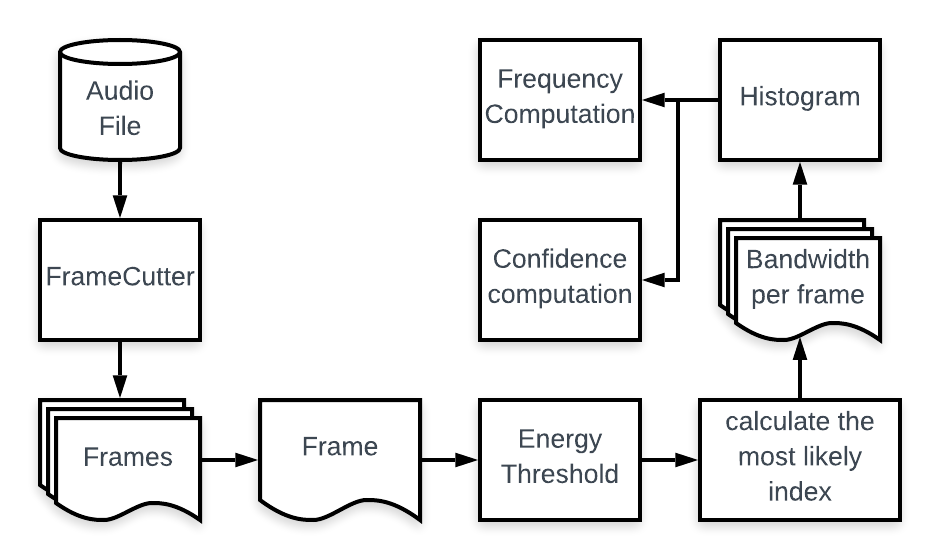
\includegraphics[clip,width=\columnwidth]{Figures/BW_Flowchart.png}% 
	\caption{Flowchart for BW detection}
	\label{fig:bwflow}
\end{figure}
The most likely bin per each frame is computed using \ref{eqn:mostlikelybin}:
\begin{equation}\label{eqn:mostlikelybin}
	Fc = max(Fc\ where\ \frac{1}{Fc}\sum_{i=Fc}^{N}FFT(x_{frame}*w_N)[i]>10^{-5} where Fc = 0,1,\dots,N)
\end{equation}
Which value and function was obtained by trying different functions that gave a stable value which to threshold. 
Once the cut frequency is computed in each frame, a weighted histogram is computed where instead of simply counting the number of occurrences 
for each frequency bin, the energy of the frame was added so that the equation results in \ref{eqn:hist}
\begin{equation}\label{eqn:hist}
	hist[f] = \sum_{i=0}^{N_{frames}}\sum_{j=0}^{N}(frame_i[j])^2\ for\ i\ so\ that\ f_i=f
\end{equation}
Where Nframes is the number of frames, N is the frame size, f is the cut frequency, fi is the extracted frequency for that frame and hist[f] 
is the histogram array in the index f.
From that weighted histogram, the most likely frequency is taken by extracting the index for which the histogram is largest.
Fc=argmax(hist) 
and the confidence is extracted in two different ways depending on the value of Fc:

From there, if the confidence value is greater than a determined threshold, defaulted to 0.8 and Fc is lower than 0.85*(N/2 +1) it is considered 
to have a problem. However, this methodology only has been explored with a frame size of 256 samples and a hop size of 128 at the moment.


\section{Low SNR defect detection}
The low SNR detection algorithm is based on the well known SNR relationship of \ref{eqn:snr}
\begin{equation}\label{eqn:snr}
	SNR = \frac{S}{N}
\end{equation}
But as the signal and the noise component of this expression, are mixed in our case, a per frame classification algorithm based on the features 
of energy and correlation was used with the following conditions: 
If a frame’s energy is less than a 10\% of the energy the frame is classified as noise. If it is higher, the next evaluation is performed.
When evaluating the correlation, the goal was to measure the resemblance of the frame to white noise. To do this, autocorrelation was used to compute it. 

\begin{figure}[!ht]
	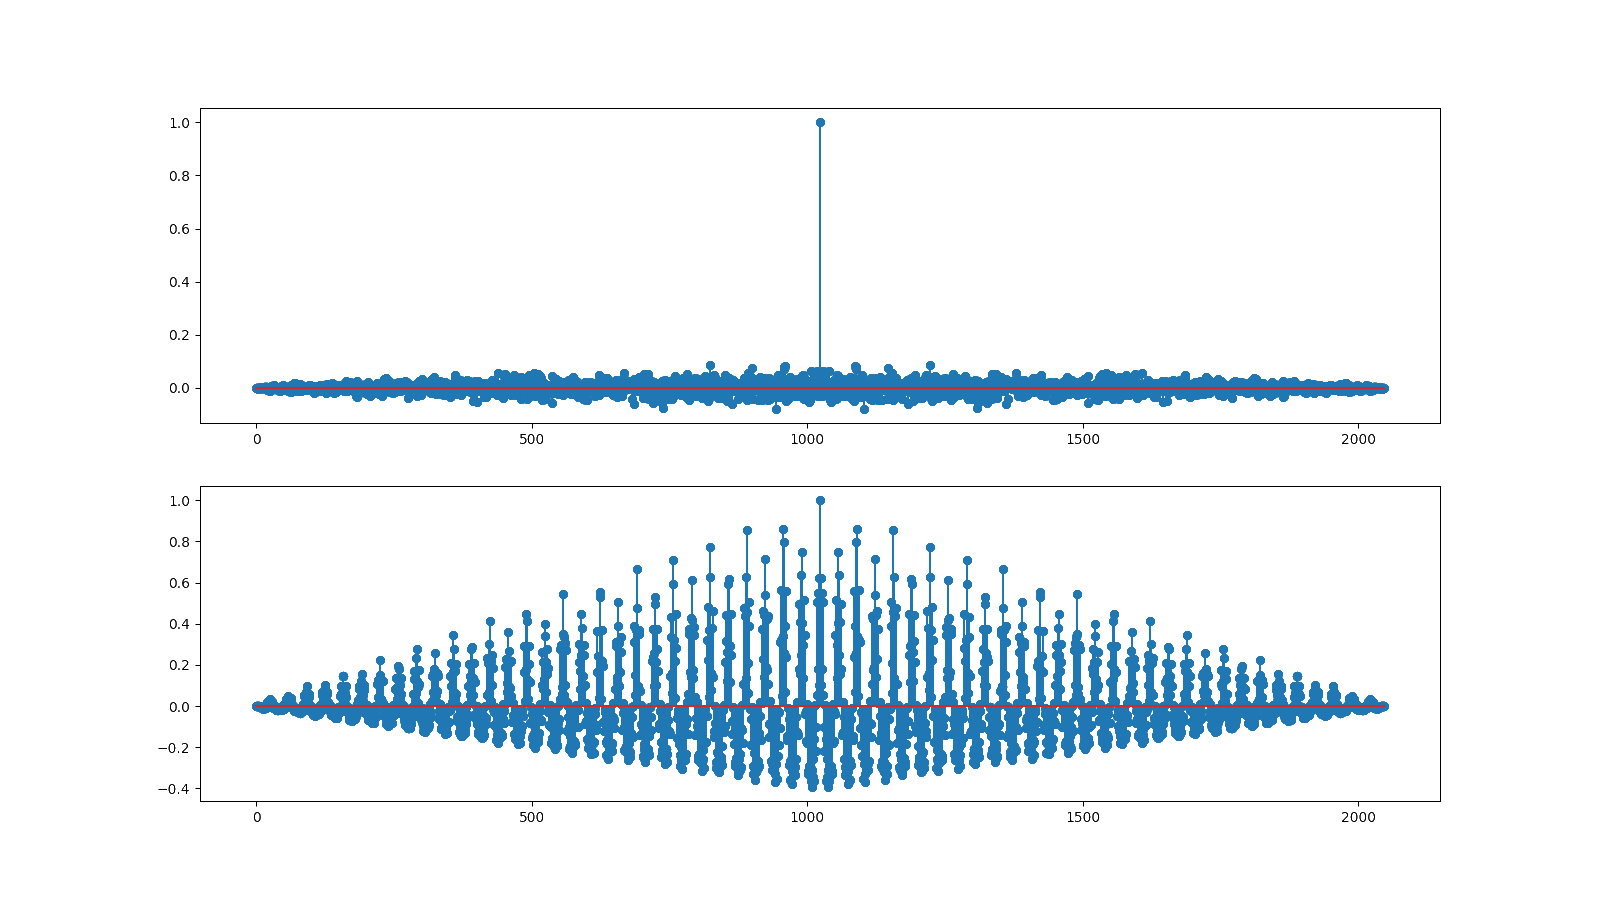
\includegraphics[clip,width=\columnwidth]{Figures/correlation.png}% 
	\caption{Autocorrelation comparison of N(0,1) noise and a more deterministic signal}
	\label{fig:accomp}
\end{figure}

Figure \ref{fig:accomp} represents an autocorrelation plot for white noise N(0,1)
and the plot below corresponds to an almost pure harmonic sound with some noise added to it. This raises the question if a measure of which 
percentage of the values lands in the sample in the middle is a good fit for a measure of similarity, which in further testing it is found that it is.
The mathematical expressions for the computation to get the value for deciding on which kind of frame we are looking at is \ref{eqn:ac}.
\begin{equation}\label{eqn:ac}
	\begin{matrix}
		R_{xx}[l]=\sum_{n=0}^{N-1}x[n]x[n-l]\\
		ac[i]=\frac{R_{xx}[0]}{\sum \left | R_{xx}[l] \right |} \ for\ i=0,1,...,N_{frames}\\ 
		ac = \frac{ac}{max(\left | ac \right |)}
	\end{matrix}
\end{equation}
This ac vector of values will give us a value between 0 and 1 for each frame which is then thresholded and if the value is lower than the threshold is 
considered signal, and noise otherwise.
From there, once the frames are classified, the power for each signal and noise frames are added and then the SNR is computed. A problem is detected if 
the SNR is higher than a threshold.

\newpage
